\documentclass[../main.tex]{subfiles}
\begin{document}

\subsection{Reeks C}
\subsubsection{Type Computers}
\begin{question}
Bespreek het onderscheid tussen mainframe, minicomputer, personal computer, werkstation, supercomputer.
\end{question}
\begin{solution}
\begin{description}
	\item[Mainframe] Mainframes zijn computers met grote capaciteit, voornamelijk gebruikt door bedrijven en overheidsinstanties, bedoeld voor het verwerken van informatie in batch. Bij een mainframe ligt de nadruk meer op ononderbroken inzet en het bedienen van een groot aantal gebruikers. Vaak zijn mainframes toegelegd op het verwerken van transacties.
	\item[Minicomputer] Een minicomputer is een klasse van computers die kleiner en goedkoper zijn dan mainframes. Ze beschikken doorgaans over in- en uitvoerapparaten en zijn in staat een hogere programmeertalen uit te voeren.
	\item[Personal computer] De personal computer is een \emph{microcomputer} voorzien van een scherm en toetsenbord. Deze computer is beduidend goedkoper dan een mainframe of minicomputer.
	\item[Werkstation] Een krachtige computer bedoeld voor professioneel gebruik. Deze computer is voorzien van gespecialiseerde hard- en software. Deze computer bevindt zich tussen de mini- en personal computer.
	\item[Supercomputer] Een supercomputer is een computer met een buitengewoon grote bewerkingscapaciteit of rekenvermogen.  Men gebruikt een supercomputer wanneer men genoegen kan nemen met een systeem dat soms uit moet voor een servicebeurt, maar waarvan absolute topprestaties verlangd worden als het systeem in bedrijf is. Daarbij ligt de nadruk meestal op \emph{floating point} bewerkingen. Vaak wordt een supercomputer gebruikt voor onderzoekswerk op universiteiten of technische instituten waarbij op ieder moment slechts een beperkt aantal mensen met het systeem werkt, en iedere gebruiker zijn eigen, specifieke applicatie heeft.
\end{description}
\end{solution}

\subsubsection{Invloed Internationale Gebeurtenissen}
\begin{question}
Toon met voorbeelden aan dat belangrijke internationale gebeurtenissen een grote rol hebben gespeeld in de ontwikkeling van computers en informatica.
\end{question}
\begin{solution}
We vinden hiervan verschillende voorbeelden terug doorheen de geschiedenis.
Reeds eind negentiende eeuw leid de grote migratie naar amerika tot het probleem van volkstellingen.
Dit gaf de aanzet tot het ontnwikkelen van de Hollerith Machine met als doel het vereenvoudigen van de volkstelling.
\\\\
Een volgende heel duidelijk voorbeeld is tijdens de tweede wereld oorlog.
Vooral in Amerika en Groot Brittanni\"e is de invloed zeer duidelijk te merken.
De Collosus I (GB) wordt in het geheim ontwikkeld om duitse geheime codes te breken.
Ook de ASCC, ENIAC (VS) van zijn opvolgers werden gebruikt door het Amerikaanse leger om o.a. projectielbanen te berekenen.
\\\\
In Duitsland was er door de oorlog vooral een negatieve invloed te merken.
Zo kreeg Konrad Zuse door de oorlogskosten geen subsidie voor het ontwikkelen van zijn Z-reeks.
Ook na de oorlog was het door gebrek aan geld en middelen relatief stil op het front van computers in duitsland.
\\\\
De ontwikkeling van het ARPAnet (voorloper van het internet) is ook gedeeltelijk toe te schrijven aan de koude oorlog.
Er was immers nood aan communicatie als er verschillende nodes in een netwerk zouden uitvallen.
\end{solution}

\subsubsection{IBM}
\begin{question}
IBM heeft een belangrijke rol gespeeld in de ontwikkeling van computers en informatica. Kan je belangrijke verwezenlijkingen of mijlpalen aangeven?
\end{question}
\begin{solution}
IBM ontstond in 1914 uit de \emph{Tabulating  Machine  Company} dat gekend is voor de \emph{Hollerith machines}. Ze groeide al snel uit tot de marktreus in gegevensverwerkende machines op basis van ponskaarten.
\begin{itemize}
	\item Havard University en IBM ontwikkelen samen in 1944 de \textbf{Harvard Mark 1}, \'e\'en van de eerste computers. Na het succes hiervan ontwikkelen ze de \textbf{Selective Sequence Electronic Calculator} (SSEC) die verschijnt in 1948.
	\item Kort na de tweede wereldoorlog verschijnt de \textbf{Card-programmed Electronic Calculator} (IBM 601/2/3/4/5). Van de IBM 605 werden er tussen 1948 en 1985 maar liefst 5000 gemaakt en verkocht.
	\item Pas vanaf 1951 ziet IBM in dat naast wetenschappelijk rekenwerk, computers ook geschikt waren voor gegevensverwerking en er een markt voor de firma bestond. In 1951 brengen ze de eerste \emph{stored program computer} uit, de \textbf{IBM 701} bedoeld voor gegevensverwerking. Omdat de gebruikte ponskaarten compatibel zijn met hun vorige apparatuur steekt IBM al snel alle concurrentie voorbij. In 1955 verschijnt de IBM 702, de business georienteerde opvolger. Deze laatste was de eerste computer die gebruik maakte van \textbf{magnetische kernen} als geheugen.
	\item Parallel met de 701 werd de IBM 650 ontwikkeld. Deze maakte gebruik van een magnetische trommel voor zijn centraal geheugen.
	\item IBM haalt een contract binnen met de US Air Force en levert 30 systemen voor SAGE (Semi-Automatic Ground Environment) waarmee IBM concurrent UNIVAC voorbijsteekt.
	\item De IBM 305 RAMAC (1956) was de eerste computer die gebruik maakte van bewegende-kop magnetische schrijven als secundaire opslag.
	\item John Backus ontwikkeling in 1957 FORTRAN voor de IBM 704 en 705.
	\item De IBM 709 (1958) introduceert als eerste een afzonderlijke processor voor I/O. Dit model wordt in 1959 vervangen door model 7090 die voorzien is van transistoren. Deze wordt opgevolgd door de 7094.
	\item Met de IBM 1400 introduceert IBM in 1960 een tweede computerserie:
	\begin{itemize}
		\item \textbf{Technisch Wetenschappelijke Toepassingen}: 700 en 1620 reeks (FORTRAN)
		\item \textbf{Administratieve Toepassingen}: 1400 reeks (COBOL)
	\end{itemize}
	\item IBM ontwikkelt APL, \'e\'en van de eerste dynamische programmeertalen.
	\item 1964: IBM wil zijn twee computerlijnen combineren. In in samenwerking met \textbf{SHARE} wordt een nieuwe programmeertaal PL/I ontwikkeld en een nieuwe familie mainframes: de \textbf{System/360}. Hoewel er verschillende versies bestaan voor verschillende gebruikers beschikken ze over dezelfde software. IBM heeft daarmee het grootste deel van de mainframe markt voor zicht. Opvolgers zijn de \textbf{System/370} in 1970, de \textbf{IBM 390} in 1985 en de \textbf{System z9} in 2006.
	\item In 1975, wordt de IBM 5100 gelanceerd, een draagbare microcomputer. Zes jaar later, in 1981 betreedt IBM de PC markt met de \textbf{IBM PC} (nidek 5150). Deze gebruikt PC-DOS als besturingssysteem en wordt al snel de de-facto standaard.
\end{itemize}
\end{solution}

\subsubsection{Computerrealisaties}
\begin{question}
60 jaar geleden: 1954. Kan je je voorstellen wat er toen nog niet was (in het dagelijkse leven), en dat gerealiseerd is door middel van computers, processoren, informatica?
\end{question}

\subsubsection{Gebeurtenissen per Decennium}
\begin{question}
Kan je een belangrijke gebeurtenis of evolutie op het gebied van de informatica voor elk decennium vanaf 1940-1949 noemen en toelichten?
\end{question}
\begin{solution}
Overzicht per decennium:
\begin{description}
	\item[Jaren 40] De Z3 is de eerste Computer. De ABC (Atanasoff Berry Computer) is de eerste computer in de USA. John von Neumann introduceert het concept van \emph{stored-program computer} dat aan de basis komt te liggen van de gehele computerindustrie. De EDSAC is de eerste werkende dergelijke computer (Groot-Brittanni\"e)
	\item[Jaren 50] De UNIVAC is de eerste commerciële computer. IBM snijdt computermarkt aan met IBm 701. Belangrijke technologische ontwikkelingen: transistor, kerngeheugen, magnetische schijven. Ontwikkeling van FORTRAN en COBOL.
	\item[Jaren 60] Verwezenlijking IC (Integrated Circuit). Samenvoegen wetenschappelijke en bedrijfsgerichte computerfamilies met System/360 van IBM. Ontstaan van minicomputers (DEC). Eerste supercomputers: Seymour Cray (CDC) met nieuwe technologie\"en als resultaat. Eerste timesharing systemen.
	\item[Jaren 70] Ontwikkeling van de microprocessor en microcomputer (IBM 5100, Apple II, Altair 8800). Vlucht microcomputers en bijhorende software (VisiCalc, WordStart). Ontwikkeling UNIX. Eerste ontwikkelingen internet.
	\item[Jaren 80] Opkomst PC en IBM 5150 met PC-DOS wordt de de-facto standaard. Evoluties hard- en software: processoren, geheugen, grafische interfaces. Ontstaan van werkstations, gepositioneerd tussen PC en minicomputer. Begin object geori\"enteerde programmeertalen (Smalltalk).
	\item[Jaren 90] Populariteit OOP neemt sterk toe (C++, Eiffel, Java). Opkomst van webgerelateerde programmeertalen (JavaScript, PHP, Python, Lua, Ruby). Start van commercieel internet en het WWW (Tim Berners-Lee), eerste browser, oprichting IETF, W3C.
\end{description}
\end{solution}

\subsubsection{Periodes}
\begin{question}
Hoe zou je zelf de geschiedenis van de informatica in periodes indelen? Op grond waarvan?
\end{question}
\begin{solution} Subjectief?
\end{solution}

\subsubsection{World Wide Web}
\begin{question}
Wat weet je over de geschiedenis en de voorlopers van het WWW?
\end{question}
\begin{solution}
Paul Otlet legde reeds in 1907 een basis voor het WWW met zijn systematische organisatie van de literatuur in de sociale wetenschappen.
Hij ontwikkelde de Universal Deciamal Classification en lag daarmee aan de basis van hypertext systemen.
In 1945 ontwierp Vannevar Bush, de wetenschappelijk adviseur van Roosevelt, het concept van een mechanisch  computer die notities en boeken gestructureerd en doorzoekbaar zou opslaan.
\\\\
Ted Nelson bedacht de term ``hypertext'' in 1965 en daarmee ook het concept Xanadu.
Hij wou alle literatuur aan elkaar linken en zo royalties uitkeren aan de originele auteurs afhankelijk van de bytes die de lezer opvroeg.
Ook wou hij een zeer eenvoudig systeem om een nieuwe versie van een tekst te publiceren en toch de oude tekst niet verloren te laten gaan.
\\\\
Er werd door de ACM een Special Interest Group on Hypertext, \emph{Hypermedia and the Web} opgericht en in 1987 werd er een eerste conferentie rond hypertext gehouden.
\\\\
In 1989 aan het CERN waren er zeer veen losse projecten lopende bijna allemaal internationaal en vaak gebruikmaken van complexe computer systemen.
Daarom stelde Tim Berners-Lee een netwerk voor.
Dit werd in 1990 werkelijkheid en info.cern.ch was een feit en het www was geboren.
\end{solution}

\subsubsection{Besturingssystemen \& Gebruikersinterfaces}
\begin{question}
Bespreek kort de evolutie van besturingssystemen en gebruikersinterfaces.
\end{question}
\begin{solution}
Een overzicht van besturingssystemen per generatie:
\begin{itemize}
	\item 1945 - 1955: Initieel bestonden er geen besturingssystemen en gebeurde programmatie rechtstreeks in machinetaal. De gebruiker en programmeur waren dezelfde persoon.
	\item 1955 - 1965: Deze generatie computers waren uitsluitend mainframes. De eerste besturingssystemen diende enkel om eenvoudig in batch programma's uit te voeren (Fortran Monitor System).
	\item 1965 - 1980: Met het samenvoegen van wetenschappelijke en administratieve computers werden besturingssystemen ingewikkeld. Timesharing vergde bovendien sterke ondersteuning van het OS.
	De eerste dergelijke systemen waren het \textbf{CTSS} (Compatible Time Sharing System) en \textbf{MULTICS} (MULTiplexed Information and Computing Service). Voor minicomputers werd MULTICS aangepast voor \'e\'en gebruiker: UNIX. Dit werd zeer populair in de academische wereld en werd later een IEEE standaard: \textbf{POSIX}.
	\item 1980 - Heden: Met de introductie van microprocessoren wordt in 1974 CP/M ontwikkeld door Gary Kindall. Het was een disk-gebaseerd besturingssysteem, beschikbaar voor meerdere processoren. In 1981 koopt Bill gates \textbf{DOS} (Disk Operating System) van Seattle Computer Products en past het aan voor IBM. Hij leverde PC-DOS samen met zijn BASIC vertolker voor IBM's Personal Computers. De PC markt bloeit en de CLI (Command Line Interface) wordt vervangen door een GUI (Graphical User Interface). Dit laatste was geinspireerd op ontwikkelingen bij Xerox PARC en gelanceerd door Steve Jobs. Microsoft volgde met Windows bovenop MS-DOS en voor UNIX verscheen X-Windows. Er ontstonden bovendien verschillende UNIX-ge\"inspireerde besturingstekens met als meest noemenswaardige Linus Torvalds \textbf{Linux}.
\end{itemize}
\end{solution}

\subsubsection{Programmeren \& Software Engineering}
\begin{question}
Hoe zijn programmeren en software engineering ge\"evolueerd?
\end{question}
\begin{solution}
Initieel werd er in de eerste generatie computers (1945-55) enkel in machinetaal geprogrammeerd.
Programmeren was toen zeer ingewikkeld en er werden vaak geavanceerde trucs toegepast.
Eind jaren 50 was er een enorme vraag naar programmeurs omdat toen computers ter beschikking van bedrijven kwamen.
\\\\
De tweede generatie (1955-65) bestond uit mainframes en werden hoofdzakelijk aangestuurd met ponskaarten.
Rond 1968 werd de term software engineering ingevoerd.
\\\\
Tussen 1965 en 1980 spreken we van een derde generatie en toen kon er voor het eerst aan multiprogramming gedaan worden.
Nu moest er ook rekening worden gehouden met time-sharing wat veel extra complexiteit meebracht en zelfs een software crisis.
\\\\
Langzaam aan won gestructureed programmeren (Hoare) aan terrein.
Unix en C maakten deze trend onder andere groot.
Bovendien was Unix een veel eenvoudiger besturingssyteem dan de complexe systemen gebruikt voor mainframes.
Eind jaren 70 werd dan de microcomputer geintroduceerd dit maakte programeren (vaak met Pascal) voor zeer veel mensen mogelijk.
\\\\
Rond 1980 werd dan OOP voorgesteld maakte het ontwerpen en implementeren van veel complexere systemen mogelijk.
Hoewel de computerkracht enorm is toegenomen wordt er slordig mee omgegaan in software.
\end{solution}

\subsubsection{Evolutie Programmeertalen}
\begin{question}
Schets de evolutie van de verschillende soorten programmeertalen aan de hand van het bijgevoegd (vereenvoudigd) overzicht. (Zie foto's voor overzicht)
\begin{figure}
		\centering
		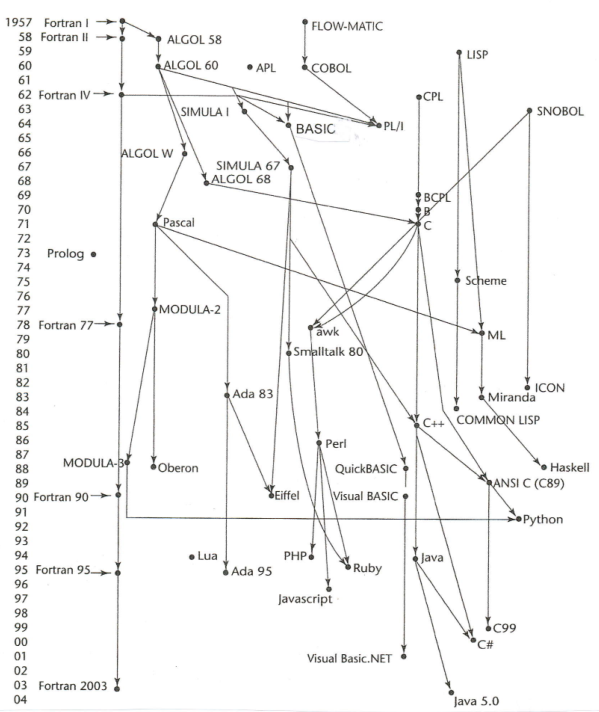
\includegraphics{overzicht_talen.png}
		\caption{(Vereenvoudigd) overzicht van de evolutie van programeertalen.}
\end{figure}
\end{question}
\begin{solution}
Initieel bestaat er enkel het imperatieve paradigma hiervoor werd er enkel in assembler of machinecode geprogrammeerd.
Initieel werden er specifieke talen ontwikkeld voor specifieke hardware.

FORTRAN I (1957) is de eerste taal met een geoptimaliseerde compiler.
De taal werd initieel ontworpen voor de IBM 704 en komt hierdoor aan zijn typerende eigenschappen.
Zo was er toen nog geen nood aan dynamische opslag, string handling of geavanceerde input/output.
Wat wel essentieel was was het behandelen van lijsten en tellende lussen waarin FORTRAN uitblonk.

FORTRAN had nog maar net zijn intrede gedaan of ALGOL werd reeds ontwikkeld.
Dit was een \emph{joint effort} om een draagbare taal te maken. Bovendien moest de taal geschikt zijn voor het beschrijven van algoritmes.
\\\\
ALGOL 58 was slechts een theoretische beschrijving en was nog niet bedoeld om ge\"implementeerd te worden.
Er was geen I/O ondersteuning maar wel een hele lijst instructies die we tot op de dag van vandaag gebruiken.
\begin{itemize}
		\item Data types (conceptueel)
		\item Subscripts binnen [haakjes]
		\item Else-If
		\item Puntkomma als statement operator: \texttt{statement;}
		\item Toekenningsoperator: \texttt{vaiable := expression;}
\end{itemize}
ALGOL 60 bevatte nog steeds werd er geen I/O ondersteund maar de taal werd wel uitgebreid met, opnieuw, elementen die we in veel hedendaagse talen terugvinden:
\begin{itemize}
		\item Blok structuur (lokale scope)
		\item Parameter passing: by value and by reference
		\item Recursie
\end{itemize}
Hoewel het  20 jaar lang de standaard was om algoritmes in te publiceren en alle volgende talen erop gebaaseerd zijn, had het weinig succes. Het gebrek aan I/O was een serieus probleem. Bovendien was de taal te flexibel wat het moeilijk maakte ze te implementeren. Bovendien zag de taal zwaar af onder de populariteit van FORTRAN en de afwezigheid van steun door IBM.
\\\\
De FLOW-MATIC taal voor de UNIVAC diende als basis voor een andere belangrijke taal in deze periode namelijk COBOL.
Het doel van deze nieuwe taal was om het aantal computer gebruikers gevoelig te verhogen.
Daarom werd er gefocust op een simpel ontwerp dat op eenvoudig Engels moest lijken.
Het ontwerp ging uit van het Amerikaanse Departement of Defense (DoD) in samenwerking met verschillende computerbedrijven.
In 1960 kwam een eerste versie uit deze bracht de volgende bekende elementen met zich mee:
\begin{itemize}
		\item Hi\"erarchische data structuren (records)
		\item Geneste selectie statements.
		\item Sterk scheiding tussen data en code.
\end{itemize}
Door het DoD raakt COBOL wijd verspreid en het werd zelfs een ANSI standaard in 1968.
\\\\
Gebruiksgemak blijft een grote drijfveer voor het ontwikkelen van nieuwe talen.
Dat bewijzen ook de ontwerp doelen van BASIC in 1963: makkelijk te leren, snel resultaat, programmeertijd minimaliseren.
Bovendien wilt men de taal gratis beschikbaar maken voor priv\'e en publiek.
Basic is sterk gebaseerd op FORTRAN en is de eerste wijdverspreide taal met de opkomst van timesharing. Tot op vandaag bestaat het populair dialect Visual Basic.
\\\\
Gedurende de jaren 60 is er een verschil tussen data verwerking en wiskundige computers.
Er was echter een groeiende vraag naar beide types en er werd dus gekeken of beiden niet konden worden gecombineerd.
Hiervoor was dan natuurlijk ook een nieuw programmeertaal nodig die zowel voor data verwerking als voor wiskundige berekeningen geschikt was en voordelen bood uit zowel FORTRAN als COBOL.
Daarom ontwierp IBM in samenwerking met SHARE PL/I in 1964
Ook hier vinden we weer bekende elementen in terug:
\begin{itemize}
	\item Exception handling
	\item Pointer data type
	\item Concurent exectution van subroutines
\end{itemize}
Midden jaren 60 wordt de basis voor Data Abstraction gelegd.
Simula 67 is sterk gebaseerd op ALGOL 60 en introduceert classes.
Verder werd er een nieuwe ALGOL 68 ontworpen die onder meer \emph{user-define data structures}, \emph{reference types} en \emph{dynamic arrays} ondersteunde.
Zelf was het geen groot succes maar het vormde wel een sterke basis voor Pascal, C en Ada.
Pascal werd ontworpen in 1971 en was weinig vernieuwd maar wel klein en gemakkelijk waardoor het vaak werd gebruikt in het onderwijs.
\\\\
In 1972 werd dan C ontwikkeld door Dennis Richie.
De taal werd speciaal voor het programmeren van operating systems ontworpen en werd zeer snel groot.
Het bood een zeer uitgebreide set aan operators aan maar bleek al snel onveilig wegens het gebrek aan type checking.
\\\\
In 1975 begon men aan het ontwerpen van Ada om zo alle verworven kennis over software engineering en language design te verzamelen.
Het werd een werk van lange adem en pas na acht jaar was de eerste volledige specificatie klaar.
Pas twee jaar later volgde een degelijke compiler.
\\\\
Ondertussen ontstond in de jaren zeventig een ander paradigma: \textbf{Object Oriented Programming}.
Xerox ontwikkelde toen immers Smalltalk wat de eerste volledige implementatie van een OOP taal was.
Xerox was een grote promotor van OOP en ook  pioniers in het design van een GUI.
In 1980 volgde de volgende belangrijke speler in OOP land gebaseerd op C: C++.
Beging jaren 90 volgde dan Java wat een enorme vereenvoudiging op C++ was.
Bovendien ook een sterke verbetering qua security.
\end{solution}

\end{document}
